%%
%% Copyright 2007, 2008, 2009 Elsevier Ltd
%%
%% This file is part of the 'Elsarticle Bundle'.
%% ---------------------------------------------
%%
%% It may be distributed under the conditions of the LaTeX Project Public
%% License, either version 1.2 of this license or (at your option) any
%% later version.  The latest version of this license is in
%%    http://www.latex-project.org/lppl.txt
%% and version 1.2 or later is part of all distributions of LaTeX
%% version 1999/12/01 or later.
%%
%% The list of all files belonging to the 'Elsarticle Bundle' is
%% given in the file `manifest.txt'.
%%

%% Template article for Elsevier's document class `elsarticle'
%% with numbered style bibliographic references
%% SP 2008/03/01
%%
%%
%%
%% $Id: elsarticle-template-num.tex 4 2009-10-24 08:22:58Z rishi $
%%
%%
%%\documentclass[preprint,12pt,3p]{elsarticle}

%% Use the option review to obtain double line spacing
\documentclass[preprint,review,12pt]{cs262}
\usepackage{amsmath}
%% Use the options 1p,twocolumn; 3p; 3p,twocolumn; 5p; or 5p,twocolumn
%% for a journal layout:
%% \documentclass[final,1p,times]{elsarticle}
%% \documentclass[final,1p,times,twocolumn]{elsarticle}
%% \documentclass[final,3p,times]{elsarticle}
%% \documentclass[final,3p,times,twocolumn]{elsarticle}
%% \documentclass[final,5p,times]{elsarticle}
%% \documentclass[final,5p,times,twocolumn]{elsarticle}

%% if you use PostScript figures in your article
%% use the graphics package for simple commands
%% \usepackage{graphics}
%% or use the graphicx package for more complicated commands
%% \usepackage{graphicx}
%% or use the epsfig package if you prefer to use the old commands
%% \usepackage{epsfig}

%% The amssymb package provides various useful mathematical symbols
\usepackage{amssymb}
\usepackage{color}

%% The amsthm package provides extended theorem environments
%% \usepackage{amsthm}

%% The lineno packages adds line numbers. Start line numbering with
%% \begin{linenumbers}, end it with \end{linenumbers}. Or switch it on
%% for the whole article with \linenumbers after \end{frontmatter}.
%% \usepackage{lineno}

%% natbib.sty is loaded by default. However, natbib options can be
%% provided with \biboptions{...} command. Following options are
%% valid:

%%   round  -  round parentheses are used (default)
%%   square -  square brackets are used   [option]
%%   curly  -  curly braces are used      {option}
%%   angle  -  angle brackets are used    <option>
%%   semicolon  -  multiple citations separated by semi-colon
%%   colon  - same as semicolon, an earlier confusion
%%   comma  -  separated by comma
%%   numbers-  selects numerical citations
%%   super  -  numerical citations as superscripts
%%   sort   -  sorts multiple citations according to order in ref. list
%%   sort&compress   -  like sort, but also compresses numerical citations
%%   compress - compresses without sorting
%%
%% \biboptions{comma,round}

% \biboptions{}

\newcommand{\note}[3]{{\color{#2}[#1: #3]}}
%\newcommand{\note}[3]{}%remove comments
\newcommand{\SERENA}[1]{\note{SERENA}{red}{#1}}
\newcommand{\MICHELLE}[1]{\note{MICHELLE}{blue}{#1}}

\usepackage{algorithm}
\usepackage{algpseudocode}
\usepackage{pifont}

\journal{CS262: Distributed Systems}

\begin{document}

\begin{frontmatter}

\title{\texttt{ConnectedHearts}: \\ A Distributed System for Viewing the Human Heartbeat}

\author[label1, label0]{Serena Booth}
\address[label1]{sbooth@college.harvard.edu}


\author[label2, label0]{Michelle Cone}
\address[label2]{mcone@college.harvard.edu}

\fntext[label0]{We, Serena Booth and Michelle Cone, affirm our awareness of the standards of the Harvard College Honor Code.}

\begin{abstract}
We present a physical distributed system for viewing the human heartbeat. We modified a medicine cabinet by embedding 13 light bulbs around the frame, as well as by replacing the cabinet's glass with one-way mirror. When a person stands in front of the cabinet, a webcam hidden behind the mirror measures their pulse. The 13 bulbs, each a virtual machine, run Bully leader election. First the leader starts pulsating with the captured pulse, and then instructs neighboring virtual machines to pulsate as well. Finally, we ensure the synchronization of the bulbs through a distributed gossip algorithm.
\end{abstract}

% \begin{keyword}
% %% keywords here, in the form: keyword \sep keyword
% example \sep \LaTeX \sep template
% %% MSC codes here, in the form: \MSC code \sep code
% %% or \MSC[2008] code \sep code (2000 is the default)
% \end{keyword}

\end{frontmatter}

%%
%% Start line numbering here if you want
%%
% \linenumbers


%% main text
\section{Introduction}
\label{sec1}

\texttt{ConnectedHearts} straddles the boundary between art and computer science. The piece is inspired by an exhibit shown around the world in modern art museums, but our re-implementation emphasizes distributed computing, as \texttt{ConnectedHearts} is a physical representation of a distributed system. We modify a retro medicine cabinet to hold 13 light bulbs around its frame. While in an ideal world each light bulb would be powered by its own microprocessor, we simulate this interaction instead by each light bulb representing a virtual machine as a process in effort to reduce expenditure. These light bulbs attempt to self-synchronize while displaying the human heartbeat. 

In this paper, we discuss the components and construction of  \texttt{Connected Hearts}, the architecture and algorithms powering the software, as well as analysis of our system. 

\subsection{Artistic Inspiration}

This piece is inspired by Rafael Lorzeno-Hemmer's ``Pulse Room''\cite{pulse} in which an entire room is outfitted with light bulbs. A physical heartbeat monitor is present in the room. A user approaches this monitor and grabs onto it. As soon as the conductance of the skin is felt, all light bulbs in the room turn off. Within a few seconds, the heartbeat monitor detects a pulse. With this, a single bulb directly above the user begins to pulsate with their heartbeat. This message is then spread to neighboring bulbs, and it bounces off of the walls; with this message-passing, the room becomes full of chaos. After a further few minutes, the bulbs synchronize, leaving the entire room pulsating with the heartbeat. We note that this system uses a single address-space to achieve this effect. 


\section{Components \& Construction}

\noindent We construct \texttt{ConnectedHearts} from the following materials:
\begin{itemize} 
\item 2 $\times$ Ubiquiti mPower Strips: 8-outlet power strips running Linux
\item Network switch and ethernet cables
\item 13 $\times$ filament bulbs and bulb holders
\item Vintage medicine cabinet, standard mirror replaced with one-way glass
\item Raspberry Pi
\item Raspberry PiCamera
\end{itemize} 

The end product looks to be a medicine cabinet with 13 light bulbs around its mirror; the majority of the components---the cables, the Raspberry Pi, etc.---are hidden from view, inside the cabinet. 

\section{System Design}


Our code is written in Python and makes extensive use of the multiprocessing library. In short, the program runs a \texttt{main.py}, the parent process. This process creates one process for running pulse detection; two more processes for turning all the relays off at the start; and 13 more processes, each corresponding to a physical light bulb. Of these 13 ``bulb'' processes, each spawns its own process to handle inter-bulb synchronization via gossip. Of these inter-bulb synchronization processes, each spawns an additional process which is tasked with maintaining the state of a continually-blinking bulb. 

\subsection{Inter-bulb Communication}

We of course do not assume the existence of a global clock. However, we do allow processes to communicate via shared memory. In particular, many processes share queues.  For example, in  \texttt{main.py}, we start up 13 ``bulb'' processes, as described above. These processes each have two process-safe queues: one of which, designated the \texttt{election\_q} stores information pertaining to leader election, and the other of which, \texttt{state\_q} stores information regarding whether the bulb should be on or off, as well as any adjustments to this, as via synchronization from gossip. 

\section{Architecture \& Algorithms}

\subsection{Pulse Detection} 

When a face is visible to a camera hidden behind the one-way glass of the medicine cabinet, we detect the pulse of the viewer. We use a Haar Classifier and OpenCV to detect the presence of a face, and we then apply code developed by NASA's Glenn Research Center\cite{NASA} to detect the pulse of the visible face. This pulse detection works by monitoring the \emph{optical intensity} of the green channel of pixels centered around the visible area of the forehead in frame. We periodically---every 30 seconds---check that a face is still visible in the scene so as to allow the user operator to change. 

\subsection{Bully: Leader Election}

Our leader election is modeled after the Bully algorithm, as originally described by Garcia-Molina in 1982 \cite{garcia1982elections}. However, we made minor modifications to this algorithm to suit our system: in our first leader election, in the way we deal with a previous leader's recovery, and in how we deal with multiple ``new election" messages.

We assume that all bulbs know all other bulbs' 64-bit uuids, assigned on program startup. We further assume that all bulbs know the layout of the system and all other bulbs' ids, ranging from 0-12, as described in Section \ref{layout}. 

Each bulb has a process-safe  \texttt{election\_q}. In our first leader election, we know that all the processes will be participating and that all uuids in the system are on their own \texttt{election\_q}. We simplify the Bully algorithm by having each process find the max uuid in its queue and choose the process with the corresponding max uuid as the leader. All the processes agree because the main thread virtually guarantees that the same uuids are put on every \texttt{election\_q}---of course, a system failure is possible, but is very unlikely. In the event of a system failure, the bulbs may disagree on a leader. 

After the leader is chosen, the other processes must make sure that it remains responsive. We achieve this by having each ``follower" ping the leader every several seconds and wait for a response. Each process is given a random \texttt{ping\_time} that determines how frequently they ping or respond to pings. This ensures that the leader is not overloaded with messages from the followers.

If a follower does not receive a response from the leader after \texttt{max\_timeout}, a time greater than the largest possible \texttt{ping\_time}, it starts a new election that follows the procedure of the Bully algorithm. It sends a ``new election" message to all processes with uuids higher than its own uuid, which causes these processes to stop pinging the leader and participate in the election. It then waits for a response from these processes for a time of \texttt{max\_timeout}. If any processes with a higher uuid respond, it waits to receive a message from a new leader. If it doesn't receive a message from a new leader within the timeout, it re-initiates a leader election. 

If a process never receives a response from a higher uuid process, or it has a higher uuid than all the responses, it assumes the role of the leader and broadcasts this message to all other processes in the system. If there is not agreement on the new leader, this procedure repeats. See Figure \ref{fig:bully} for a diagram of how this works in our system. After the broadcast from the new leader, all the followers begin pinging it and it responds to their pings. If a follower does not receive a response, then leader election starts again.\\ \textbf{Our Implementation Differences}

In our leader election, while a process waits for a response from all higher uuid processes, it also checks for ``new election" messages. If it receives a ``new election" message, it sends its uuid to the appropriate processes and continues waiting to hear back from the higher uuid processes.

If a process every receives a ``new leader" message while it is pinging the leader, it starts a new leader election.

To allow a process that was previously a leader to recover from a crash, the current leader pings any higher uuid processes with a ``new leader" message every \texttt{ping\_time}.

\begin{figure}[t!]
  \centering
  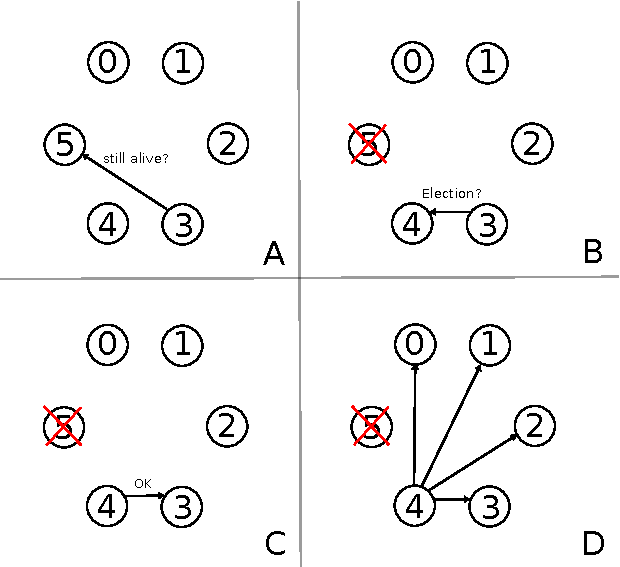
\includegraphics[width=0.7\textwidth]{figures/bully}
  \caption{In the above graphic, we demonstrate the bully algorithm for determining a leader. In sub-image A, node 3 attempts to confirm that the known leader, node 5, is still alive. In sum-image B, node 5 does not respond to node 3 for a set period of time---a time set by node 3. Hence node 3 initiates an election by contacting all nodes with a higher id than itself. In sub-image C, node 4 responds to node 3's request to initiate an election by confirming it remains alive. Finally, in sub-image D, node 4 broadcasts a message to all nodes to inform them of its leader status. 
 \label{fig:bully}}
\end{figure} 


\subsection{Realtime Synchronization via Gossip}

In our system, each ``bulb'' process has its own SSH connection to the Linux Ubiquiti box by which it is powered. This process repeatedly sends message to the box of the form \texttt{echo X > /proc/power/relayY}, where \texttt{X} $\in \{0,1\}$, and \texttt{Y} represents the id of the relay controlling the power supply to the box. Commands to turn the box on are followed by some amount of wait, determined by the user's pulse, followed by a command to turn the box off and wait. However, as our system is ``distributed,'' and we have no concept of a global time, the bulb relay switches are poorly aligned lacking any inter-process synchronization. We thus implement a simple gossip algorithm, as inspired by Babaoglu et al, \cite{babaoglu2007firefly}. 

Given that the physical layout of our system is fixed, we can select the more \emph{trustworthy} of our neighbors, an algorithm which we describe below. With this neighbor, we attempt to iteratively align our synchronization over time. This algorithm is further described in Algorithm \ref{CHalgorithm}. 

\begin{algorithm}
\caption{Synchronization via Gossip}
\label{CHalgorithm}
\begin{algorithmic}[1]
\Procedure{Gossip}{}
\While {True} 
\State Receive messages from \{trustworthy neighbor, self\}
\If{diff(self\_time, neighbor) $<$ diff(self\_time, neighbor + bpm)}
\State Increase wait (while bulb off)
\Else
\State Decrease wait (while bulb on)
\EndIf
\EndWhile
\EndProcedure
\end{algorithmic}
\end{algorithm}

We note that in order to run this gossip procedure, we require a bulb control process to receive a message from its trusted neighbor, as well as from its own child process. When this does not happen, the amount of wait time is based solely on the pulse. On the other hand, when this bulb does received these communications, an invariant enforces that the bulb receives a message from its trusted neighbor before receiving a message from itself. 
\\

Given the following scenario, assuming that the pulse rate is $\frac{1}{2}$ second: 

$$ \text{A) Trusted neighbor:  00:01}$$
$$ \text{B) Trusted neighbor:  00:02}$$
$$ \text{C) Trusted neighbor:  00:03}$$
$$ \text{D) Self:  00:04}$$

The process would ignore messages (A) and (B). It would consider message (C), message (D), as well as a calculated message (E): $\text{E} = \text{C} + 2 * \frac{1}{2} $, which estimates the time when the trusted neighbor will send its next message, based on the rate of the pulse. The process would then determine whether its own signal was closer to the trusted neighbor's previous time or if it was closer to the trusted neighbor's expected future time. In case of the former, the bulb would affect the rate of its blinking by waiting for \emph{less} time while in the ON state; in the latter, the bulb would affect its rate by waiting for \emph{more} time while in the OFF state. If the times of the messages are sufficiently close, the bulb will not adjust its rate of blink. 


\subsubsection{Physical Layout}
\label{layout}

\begin{figure}[h]
  \centering
  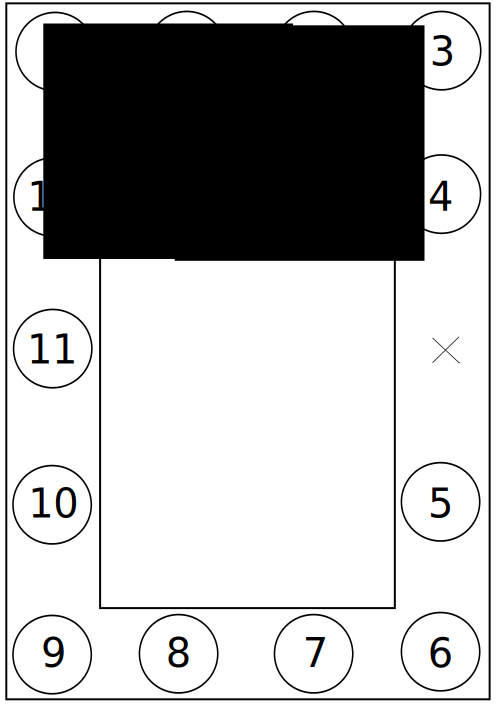
\includegraphics[width=0.3\textwidth]{figures/system_layout}
  \caption{The system layout. While each bulb is assigned a 64-bit uuid during the program, each bulb also has an id, shown above, ranging from $0-12$, which allows the system to consistently converge toward the leader bulb's rate of pulsation during the synchronization routine. 
 \label{fig:layout}}
\end{figure}

The physical layout of our system is predetermined, as shown in Figure \ref{fig:layout}. Each bulb is assigned a fixed, position-based id as well as the formerly discussed, generated 64-bit uuid. Because of this fixed layout, we are able to personalize gossip for synchronization in order to ascribe neighboring processes with scores of \emph{trustworthiness}. As the leader bulb initiates the heartbeat pulsation, the leader is the single most trustworthy bulb. This has implications for all other bulbs, however: as bulbs increase in distance from the leader, a known measure based on the system's fixed layout, their trustworthiness decreases. Thus when a bulb is receiving contradictory gossip from its two neighboring bulbs, it prioritizes the message which was sent by the bulb closer to the leader.  

\section{Synchronization Testing \& Analysis}

\begin{figure}
\thispagestyle{empty}
\vspace{-10 mm}
  \centering
    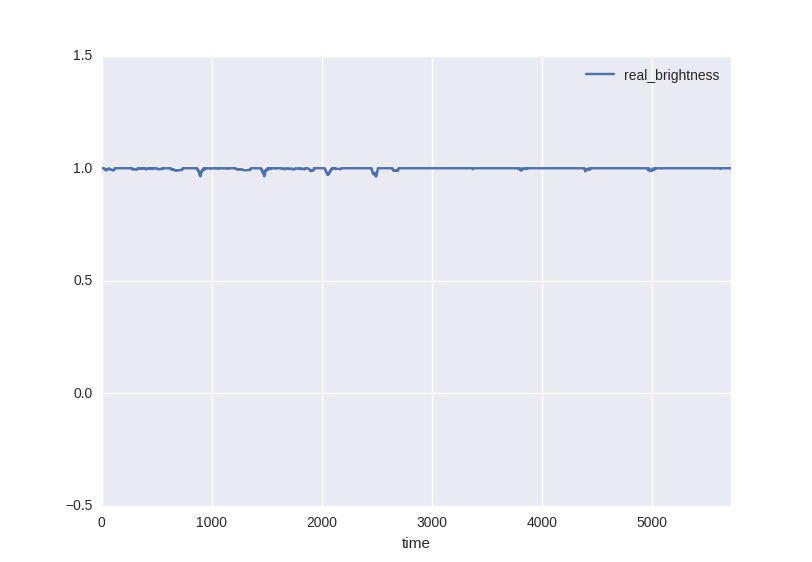
\includegraphics[width=0.9\textwidth]{figures/bad_synch.png}
  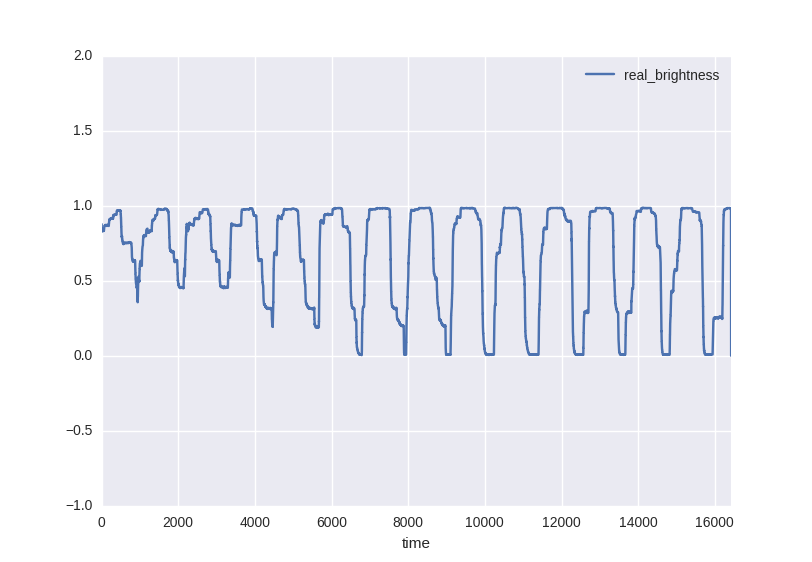
\includegraphics[width=0.9\textwidth]{figures/graph_well_synched.png}
  \caption{With heartbeat 50bpm, we demonstrate the synchronization of our system as a function of time. Above: the system in the absence of any gossip. The average brightness in the scene is consistently extremely high. Below: we run synchronization via gossip. The system starts out somewhat desynchronized, so the average brightness values of the system range from 0.4 to 1. Once the system is synchronized, the values range neatly from 0 to 1, the full possible range. 
 \label{fig:res}}
\end{figure}

In order to analyze the success of our synchronization via gossip, we implement a simple computer vision system. The steps of analysis are as follows: 

\begin{enumerate} 
\item We capture footage at a high-frame rate. 

- 120 fps; however, we note that this frame rate is slower than the processing rate of the human eye. 

\item With GUI, present user with first frame of the captured footage. 

- User selects 13 pixels corresponding to bulb filaments. 

\item Brightness timeseries computed. 

- The brightness of these pixels are averaged for every frame in the video, and ultimately we produce a timeseries of this brightness data.
\end{enumerate}

In Figure \ref{fig:res}, we run this analysis procedure on our system without gossip and then with gossip. When we run the system without gossip, the system appears to be very bright for its entire operation. This is because, when a bulb is on, it illuminates its neighboring bulbs, which have reflective surfaces. Thus, to the camera, it is impossible to discern between one bulb or three bulbs being on. Due to the lack of synchronization in the absence of gossip, at all points in the operation, at least every other fourth bulbs is on at the same time, making the system appear to be entirely on for the full duration of the clip. 


\section{Conclusion}

The final product of \texttt{ConnectedHearts} exceeded our expectations: while we were originally unsure that gossip could be achieved given the unreliability of some of our components, we found that, to a rate of 120 frames-per-second, the visual appearance of the mirror is indeed synchronized. Over the course of this project, we learned a substantial amount about distributed systems, some of which we relay here: 

\begin{enumerate}
\item Debugging a (fake!) distributed system is hard, and the separation between unreliable hardware and buggy code can be indecipherable. 

One intriguing aspect of our system is our dependence on unreliable Linux boxes. Due to the presence of these unreliable machines, debugging our implementation of gossip was extremely challenging. 

\item Referring to the same memory address between different processes without use of locks is erroneous; using process-safe objects is extremely important when sharing memory between processes.

We encountered a bug that took several hours to unravel where all the processes shared a queue that we were sure had the same memory address. Despite this, when something was successfully added to the queue by one process, only that process was able to see the change in the queue. The queue was a non process safe \texttt{Queue.Queue}. After switching to a \texttt{multiprocessing.queues.Queue}, the problem disappeared and the processes were able to correctly share the queue.
\end{enumerate}

\subsection{Future Work} 

While the synchronization of our heartbeat visualization is visually appealing when synchronizing via gossip, the precision of control we have is relatively poor. Instructions to turn relays on or off are sent over SSH connections; the amount of time required for this may vary, and may not be internally consistent. 

A future improvement to this work could be to create a closed feedback loop. Instead have a process dispatch an SSH command to a Linux powerstrip and then send a message to another process indicating that the bulb has flashed with the heartbeat, we could position the camera internal to the mirror in such a way as to allow it to directly view the bulbs. Instead, then, of guessing when the physical bulb turned on, we could know precisely when it did so and only send a message indicating this when appropriate. 

\subsection{Sap}

Serena is graduating in two weeks, and this project was her last piece of coursework at Harvard; an incredibly high note to end her time here! 

Michelle is graduating in a year, but is really sad that this class is now over and she won't get to listen to Professor Waldo's hilarious lectures anymore.



%% The Appendices part is started with the command \appendix;
%% appendix sections are then done as normal sections

%% References
%%
%% Following citation commands can be used in the body text:
%% Usage of \cite is as follows:
%%   \cite{key}         ==>>  [#]
%%   \cite[chap. 2]{key} ==>> [#, chap. 2]
%%

%% References with bibTeX database:

\bibliographystyle{elsarticle-num}
% \bibliographystyle{elsarticle-harv}
% \bibliographystyle{elsarticle-num-names}
% \bibliographystyle{model1a-num-names}
% \bibliographystyle{model1b-num-names}
% \bibliographystyle{model1c-num-names}
% \bibliographystyle{model1-num-names}
% \bibliographystyle{model2-names}
% \bibliographystyle{model3a-num-names}
% \bibliographystyle{model3-num-names}
% \bibliographystyle{model4-names}
% \bibliographystyle{model5-names}
% \bibliographystyle{model6-num-names}

\bibliography{sample}


\end{document}

%%
%% End of file `elsarticle-template-num.tex'.
